\documentclass[aspectratio=169]{beamer}

% ---------- THEME & LOOK ----------
\usetheme{Madrid}
\usecolortheme{seahorse}
\usefonttheme{professionalfonts}
\setbeamertemplate{navigation symbols}{}
\setbeamercovered{transparent}
\setbeamertemplate{itemize items}[circle]
\setbeamertemplate{enumerate items}[default]
\setlength{\parskip}{0.25em}

% ---------- COLORS ----------
\usepackage{xcolor}
\definecolor{accent}{RGB}{0,92,184}
\setbeamercolor{structure}{fg=accent}
\setbeamercolor{title}{fg=white,bg=accent}
\setbeamercolor{frametitle}{fg=accent}
\setbeamercolor{block title}{bg=accent!10,fg=accent}
\setbeamercolor{block body}{bg=accent!3}

% ---------- PACKAGES ----------
\usepackage{booktabs}
\usepackage{amsmath, amssymb}
\usepackage{array}
\usepackage{hyperref}
\hypersetup{colorlinks=true,linkcolor=accent,urlcolor=accent}

% ---------- PLACEHOLDER BOX (compile-safe; no images required) ----------
\newcommand{\placeholderbox}[2][0.82\linewidth]{%
  \begin{center}
    \fbox{\begin{minipage}[c][0.46\textheight][c]{#1}
      \centering \vspace{0.25em}
      \textbf{#2}\\[0.6em]
      \emph{Insert figure/diagram here later.}
    \end{minipage}}
  \end{center}
}

% ---------- TITLE ----------
\title{\textbf{Labour Supply -- Individual Attachment to the Labour Market \vspace{.5cm}\\  }}
\subtitle{ {\large ECON 300 - Labour Economics}}
%\institute{UNBC}
\author{Muhebullah Karimzada}

\date{Winter 2026}



\begin{document}

% ============================================================
% TITLE
% ============================================================
\begin{frame}[plain]
  \titlepage
\end{frame}

% ============================================================
\section{Orientation}
% ============================================================

\begin{frame}{Learning Objectives}
\transfade
\begin{itemize}[<+->]
  \item Define employment, unemployment, labour force participation, and hours worked; understand Statistics Canada measurement and reporting.
  \item Use the income–leisure model to show trade-offs in whether and how much to work.
  \item Distinguish individual choices from the opportunity sets available.
  \item Decompose wage changes into income and substitution effects and interpret ambiguous net responses.
  \item Apply the model to married women’s labour supply decisions.
\end{itemize}

\end{frame}

\begin{frame}{Main Questions}
\transfade
\begin{itemize}[<+->]
  \item How do we measure labour market attachment, and how has it evolved?
  \item Where does participation fit within labour supply theory?
  \item How do men’s and women’s labour supply decisions differ and why?
  \item Should labour supply increase with the market wage? What does theory say?
  \item What does the evidence show about wage responsiveness?
  \item Why do firms pay an \textit{overtime premium} instead of just a higher straight-time wage?
\end{itemize}

\end{frame}

% ============================================================
\section{Measuring Labour Market Attachment}
% ============================================================

\begin{frame}{Quantifying Labour Market Attachment}
\transfade
\textbf{Labour Force (LF):} Eligible population (15+) who are employed or unemployed.\\
\textbf{LF Participation Rate (LFPR):} Fraction of eligible population in LF; \(\text{LFPR} = \frac{\text{LF}}{\text{POP}}\).
\begin{block}{Student Tip}
Keep POP (eligible), LF (in the game), and those \textit{outside} LF distinct; misclassification drives measurement issues.
\end{block}

\end{frame}

\begin{frame}{Unemployment (Definition)}
\transfade
To be \textbf{unemployed}, a person must be in one of:
\begin{enumerate}[<+->]
  \item Without work and actively searched in the last 4 weeks,
  \item Waiting to be recalled from layoff,
  \item Waiting to start a job within 4 weeks.
\end{enumerate}

\end{frame}

\begin{frame}{Figure 2.1: Labour Force Concepts (Jan 2020) }
\centering
\vspace{2em}

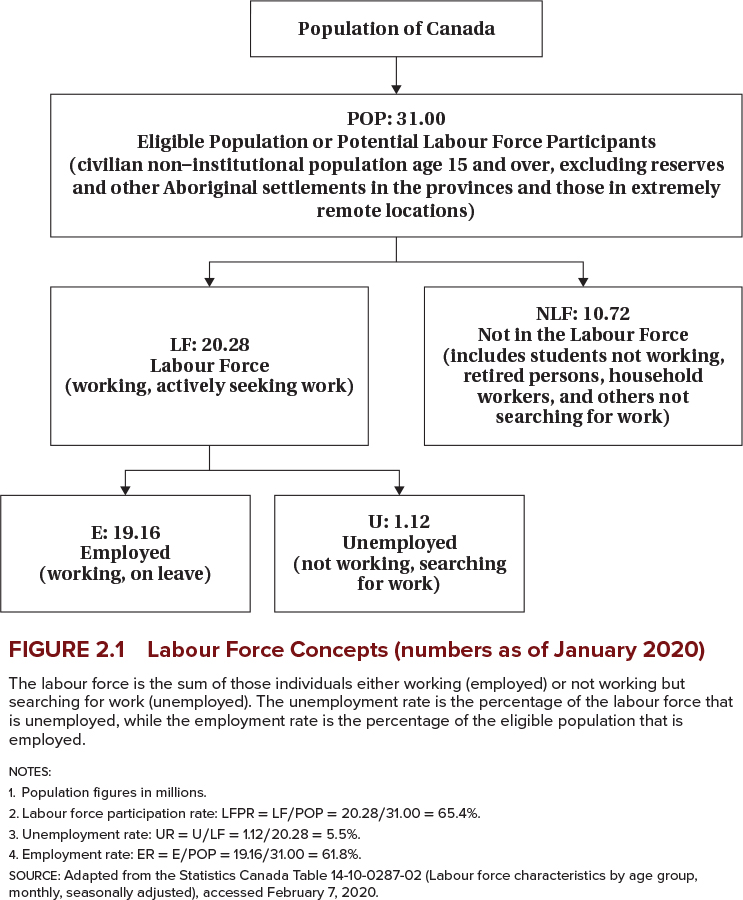
\includegraphics[width=0.52\linewidth]{ben54842_0201}.

\end{frame}

\begin{frame}{Figure 2.2: LF Participation Rates by Sex, Canada, 1901–2019 }
\centering
\vspace{2em}

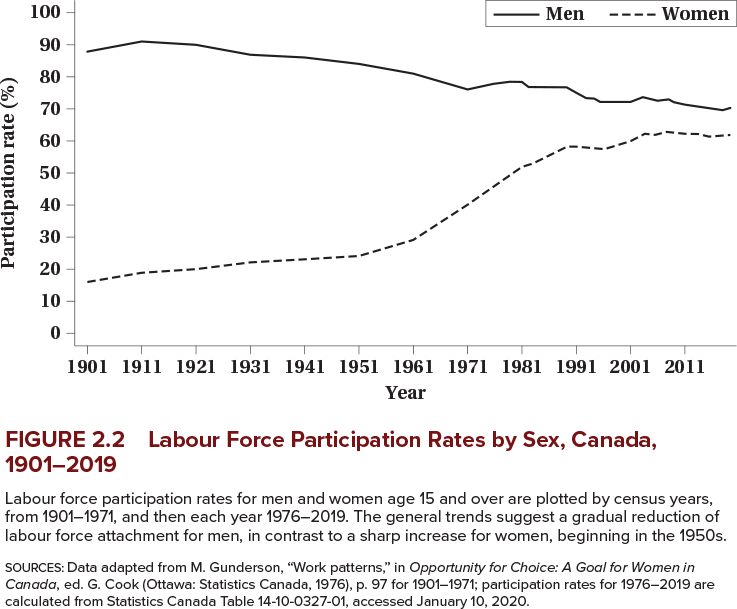
\includegraphics[width=0.77\linewidth]{ben54842_0202}.

\end{frame}

\begin{frame}{TABLE 2.1: Labour Force Participation Rates by Sex, Selected Countries, 2018}
\transfade
\scriptsize
\begin{tabular}{lcccc}
\toprule
\textbf{Country} & \textbf{Abbrev.} & \textbf{Overall} & \textbf{Male} & \textbf{Female} \\
\midrule
Sweden & SWE & 82.9 & 84.8 & 81.0 \\
Vietnam & VNM & 82.7 & 86.4 & 79.1 \\
Peru & PER & 80.3 & 887.2 & 73.3 \\
Canada & CAN & 78.5 & 81.9 & 75.1 \\
United Kingdom & GBR & 77.5 & 82.2 & 72.8 \\
Norway & NOR & 77.3 & 79.2 & 75.2 \\
Russia & RUS & 74.1 & 79.8 & 68.9 \\
Jamaica & JAM & 72.4 & 78.0 & 66.9 \\
United States & USA & 72.3 & 77.7 & 66.8 \\
France & FRA & 71.7 & 75.8 & 67.5 \\
Kenya & KEN & 66.9 & 69.6 & 64.1 \\
Italy & ITA & 65.3 & 74.9 & 55.7 \\
Mexico & MEX & 64.7 & 82.6 & 47.1 \\
Philippines & PHL & 62.0 & 76.2 & 47.7 \\
Bangladesh & BGD & 61.1 & 83.9 & 38.1 \\
South Africa & ZAF & 59.6 & 66.0 & 53.4 \\
Nigeria & NGA & 55.2 & 59.9 & 50.5 \\
Egypt & EGY & 51.1 & 76.9 & 24.7 \\
Jordan & JOR & 41.6 & 67.4 & 15.1 \\
\bottomrule
\end{tabular}

\vspace{0.25em}
\scriptsize \textit{Difference} column referenced in text is (Male - Female). Values as shown in chapter table. 
\end{frame}

\begin{frame}{Figure 2.3: Male and Female Participation vs.\ Development}
\centering
\vspace{2em}

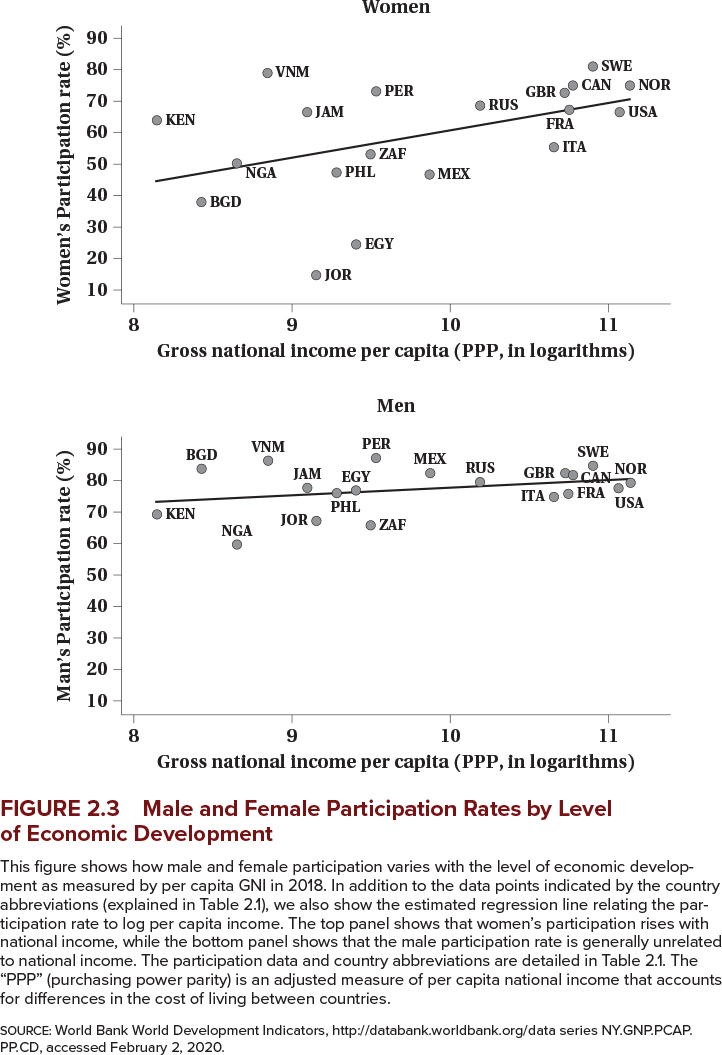
\includegraphics[width=0.41\linewidth]{ben54842_0203}.
\end{frame}

\begin{frame}{Hours-of-Work}
\transfade
\begin{itemize}[<+->]
  \item Hours per day, days per week, weeks per year.
  \item Affects the \emph{quantity} and \emph{quality} of labour supply.
\end{itemize}

\end{frame}

\begin{frame}{Figure 2.4: Distribution of Hours Worked Per Week by Sex, 2019 }
\centering
\vspace{2em}

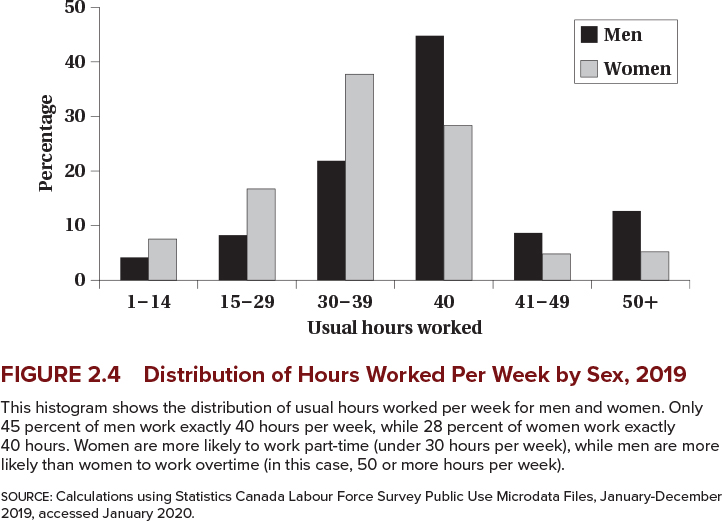
\includegraphics[width=0.89\linewidth]{ben54842_0204}.

\end{frame}

% ============================================================
\section{The Income–Leisure Model}
% ============================================================

\begin{frame}{Basic Income–Leisure Model}
\transfade
Choice of hours worked given opportunities and value of non-market time:
\begin{itemize}[<+->]
  \item \textbf{Preferences \& Constraints}
  \item Individuals choose the feasible outcome that maximizes satisfaction.
\end{itemize}

\end{frame}

\begin{frame}{Preferences}
\transfade
Two goods: \textbf{Consumption} and \textbf{Leisure}; represented by indifference curves.
\begin{itemize}[<+->]
  \item Well-defined preferences imply every bundle lies on some indifference curve.
  \item Indifference curves show combinations yielding equal utility.
  \item \(\left| \text{slope} \right| = \text{MRS}\): leisure accepted per unit of consumption foregone.
\end{itemize}

\end{frame}

\begin{frame}{Figure 2.5: Consumption–Leisure Indifference Curves }

\centering
\vspace{2em}

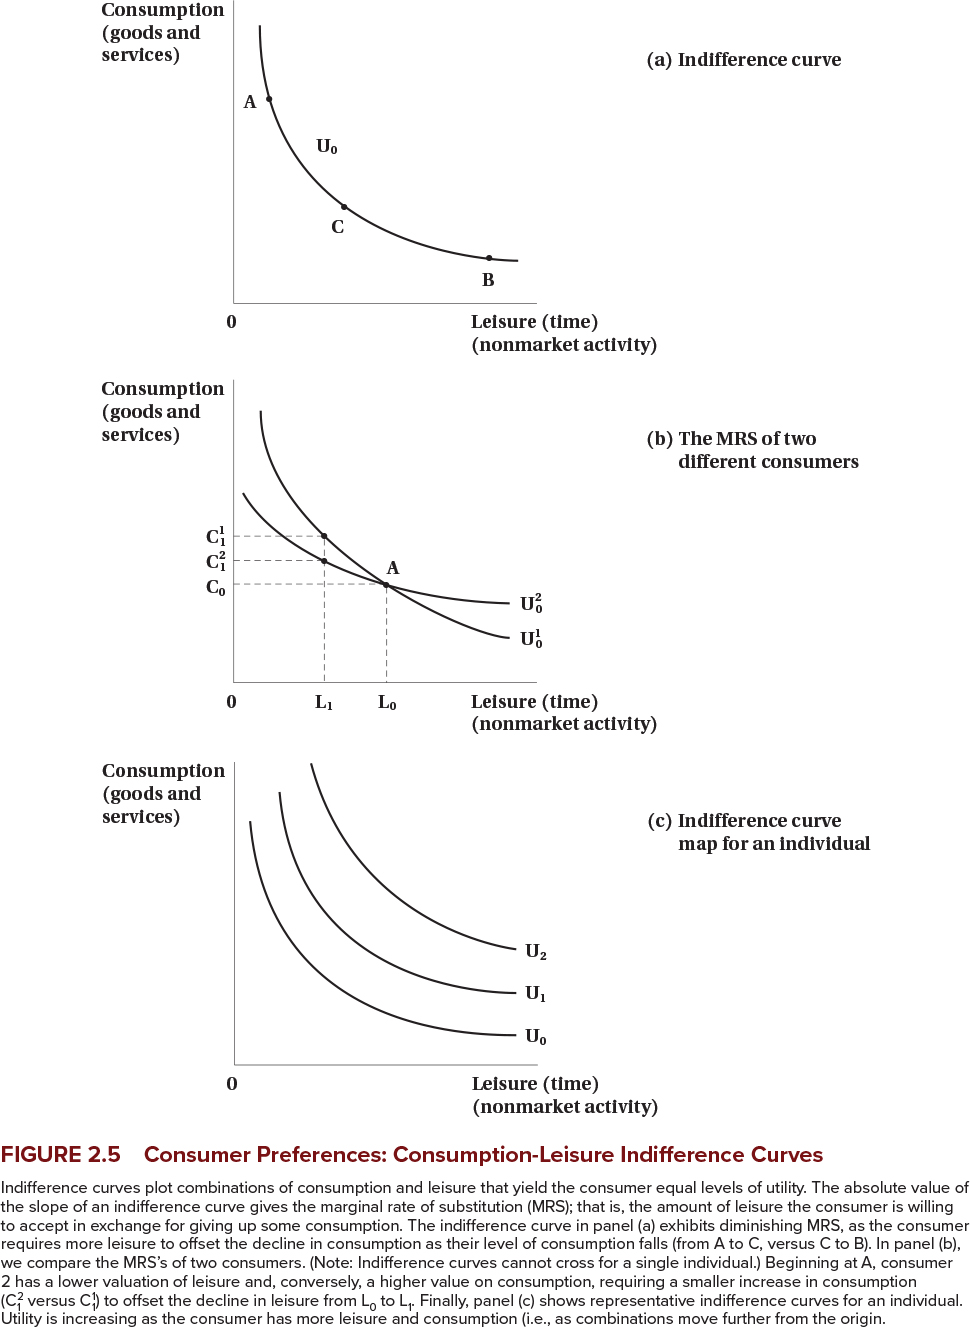
\includegraphics[width=0.385\linewidth]{ben54842_0205}.
\end{frame}

\begin{frame}{Constraints}
\transfade
\begin{itemize}[<+->]
  \item Market sets price of consumption; transforms consumption–leisure into \textbf{income–leisure}.
  \item Potential income (budget / full-income) constraint defines feasible set of income–leisure combinations.
\end{itemize}

\end{frame}

\begin{frame}{Figure 2.6: Potential Income Constraints}
\centering
\vspace{2em}

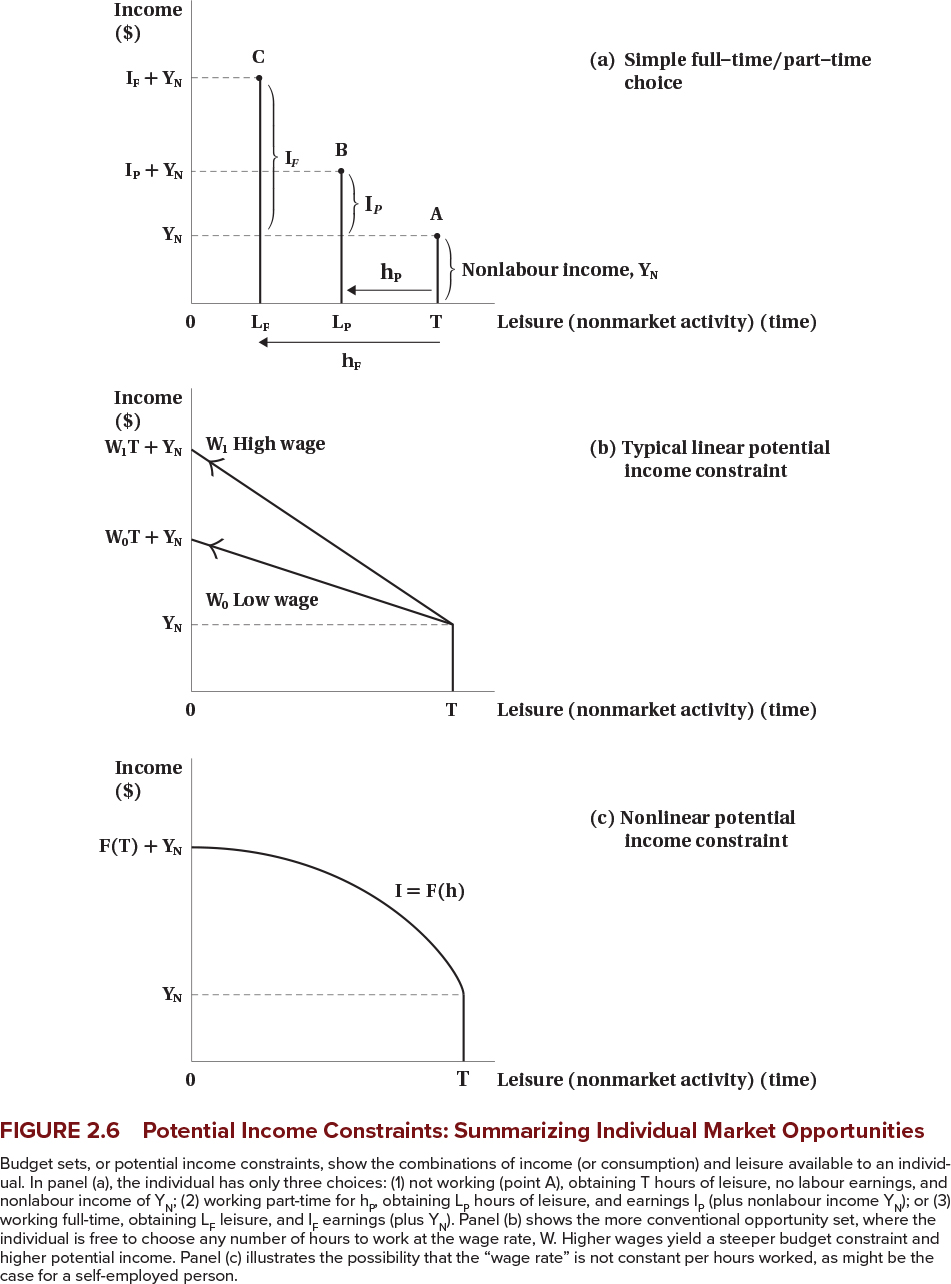
\includegraphics[width=0.385\linewidth]{ben54842_0206}.

\end{frame}

\begin{frame}{The Consumer’s Optimum}
\transfade
Optimal income and leisure at the highest indifference curve tangent to the income constraint.
\begin{itemize}[<+->]
  \item Compare \textbf{MRS} (willingness to trade leisure for income) with the \textbf{market wage} (ability to trade).
\end{itemize}

\end{frame}

\begin{frame}{Figure 2.7: The Consumer’s Labour Supply Decision}
\centering
\vspace{2em}

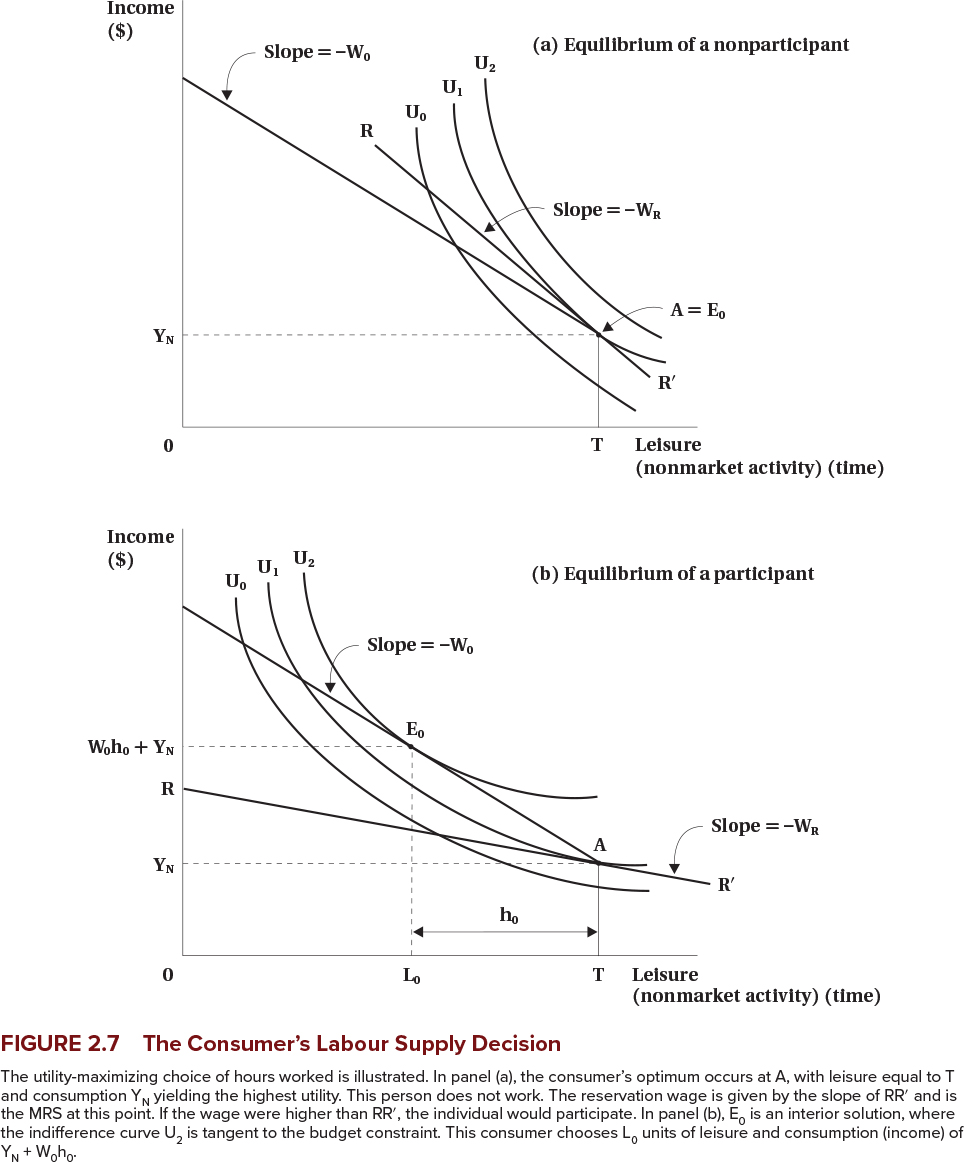
\includegraphics[width=0.42\linewidth]{ben54842_0207}.

\end{frame}

\begin{frame}{Worked Example: Part-Time Work at University}
\transfade
\small
Jack and Jill each have a weekly allowance of \$100 and can work at \$10/hour. They have 98 discretionary hours (after 10 hours/day personal needs).\\[0.3em]
\textbf{Budget line:} \(C = 100 + 10H\), where \(H\) is hours worked; leisure \(L = 98 - H\).\\
\textbf{Interpretation:} Intercepts at \(C=100\) (no work) and \(H=98\) hours $\rightarrow$  \(C=100+10(98)=1080\).\\
\textbf{Use case:} Place indifference curves to show who works more given identical opportunities but different preferences for leisure vs.\ consumption.

\end{frame}

\begin{frame}{Worked Example: Part-Time Work at University}

\centering


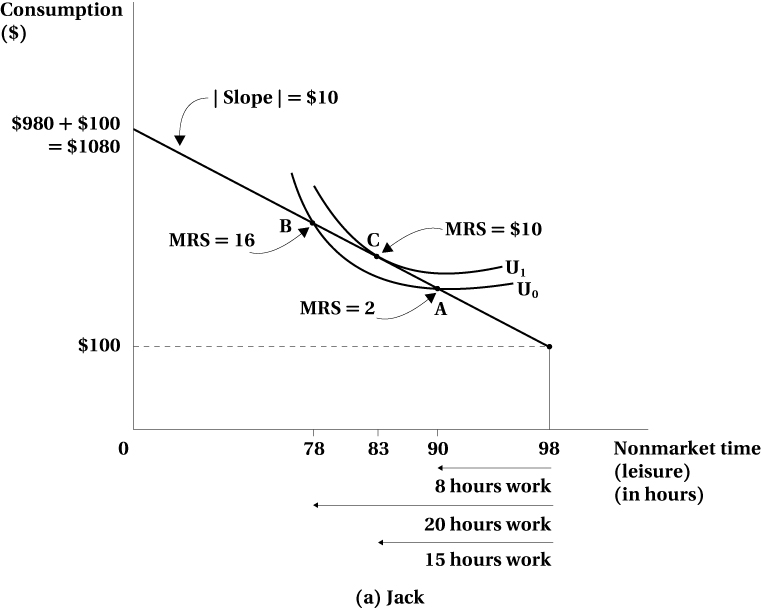
\includegraphics[width=0.56\linewidth]{ben54842_un0201a}.
\end{frame}


\begin{frame}{Worked Example: Part-Time Work at University}

\centering


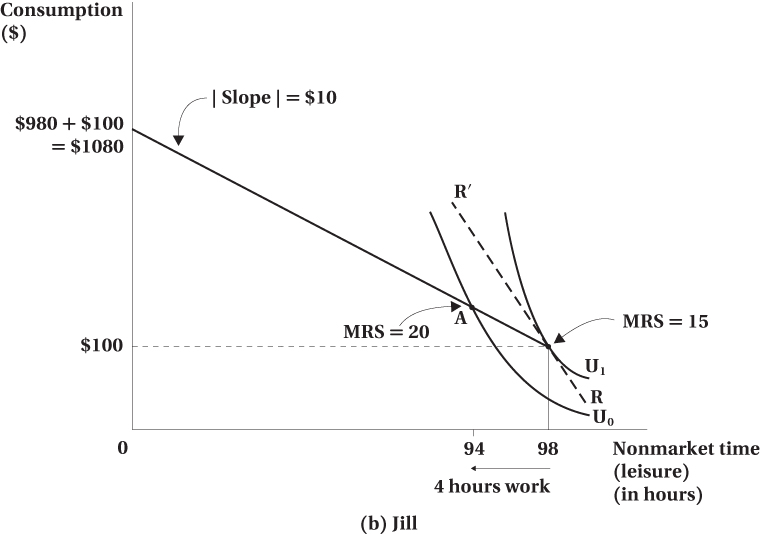
\includegraphics[width=0.56\linewidth]{ben54842_un0201b}.
\end{frame}


% ============================================================
\section{Comparative Statics}
% ============================================================

\begin{frame}{Non-Labour Income and Hours}
\transfade
Increase in non-labour income shifts the budget constraint outward (parallel).
\begin{itemize}[<+->]
  \item If leisure is \textbf{normal}, consume more leisure \(\Rightarrow\) fewer hours.
  \item If leisure is \textbf{inferior}, consume less leisure \(\Rightarrow\) more hours.
\end{itemize}

\end{frame}

\begin{frame}{Figure 2.8: Increase in Non-Labour Income}
\centering
\vspace{2em}

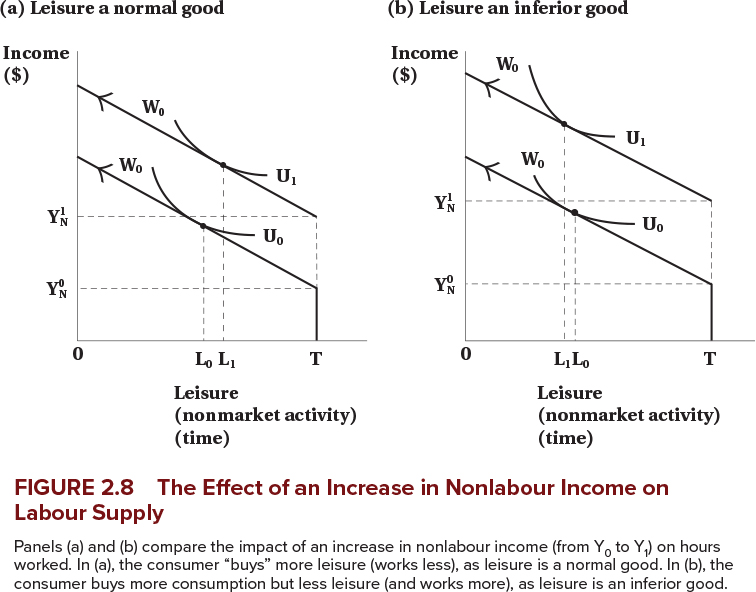
\includegraphics[width=0.71\linewidth]{ben54842_0208}.

\end{frame}

\begin{frame}{Wage Changes: Income vs.\ Substitution Effects}
\transfade
\begin{itemize}[<+->]
  \item \textbf{Income effect:} Higher wage \(\Rightarrow\) higher income \(\Rightarrow\) more leisure (fewer hours).
  \item \textbf{Substitution effect:} Higher wage raises price of leisure \(\Rightarrow\) substitute toward work (more hours).
  \item Net effect on hours is \textbf{ambiguous}.
\end{itemize}
\end{frame}

\begin{frame}{Figure 2.9: Decomposing a Wage Increase}
\centering
\vspace{2em}

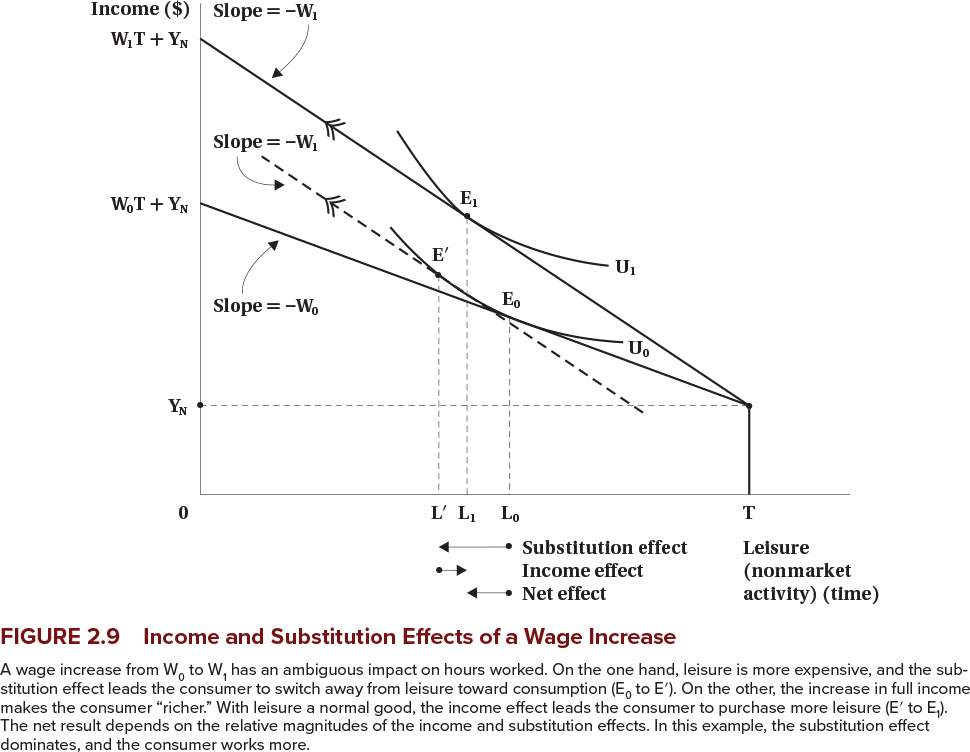
\includegraphics[width=0.7\linewidth]{ben54842_0209}.

\end{frame}

\begin{frame}{Participation Effects of Wage Changes}
\transfade
\begin{itemize}[<+->]
  \item For a non-participant, higher wage can induce entry if it exceeds reservation wage.
  \item For participants, hours may rise or fall depending on which effect dominates.
\end{itemize}

\end{frame}

\begin{frame}{Figure 2.10: Wage Increase and Participation }
\centering
\vspace{1.7em}

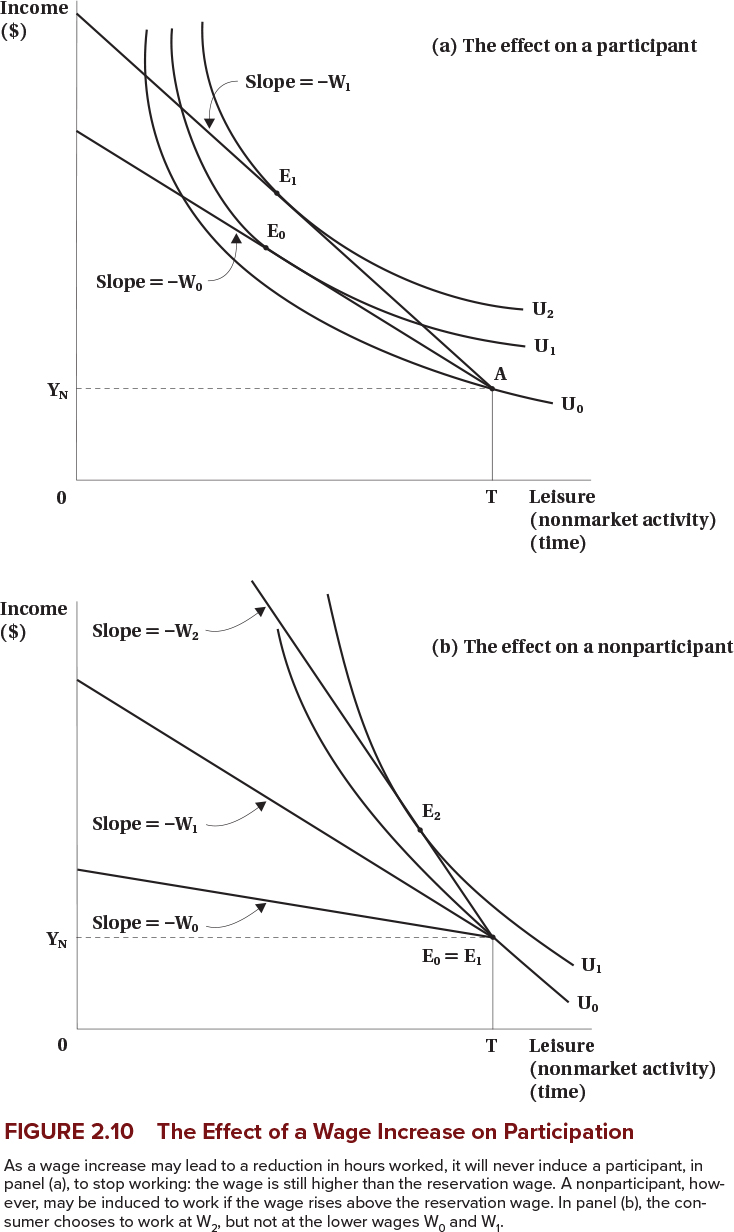
\includegraphics[width=0.3\linewidth]{ben54842_0210}.
\end{frame}

\begin{frame}{Deriving the Individual Labour Supply Curve}
\transfade
If substitution effect dominates at low wages, hours increase with wage; at higher wages, income effect can dominate, producing a \textbf{backward-bending} segment.

\end{frame}

\begin{frame}{Figure 2.11: Individual Labour Supply Curve }
\centering
\vspace{2em}

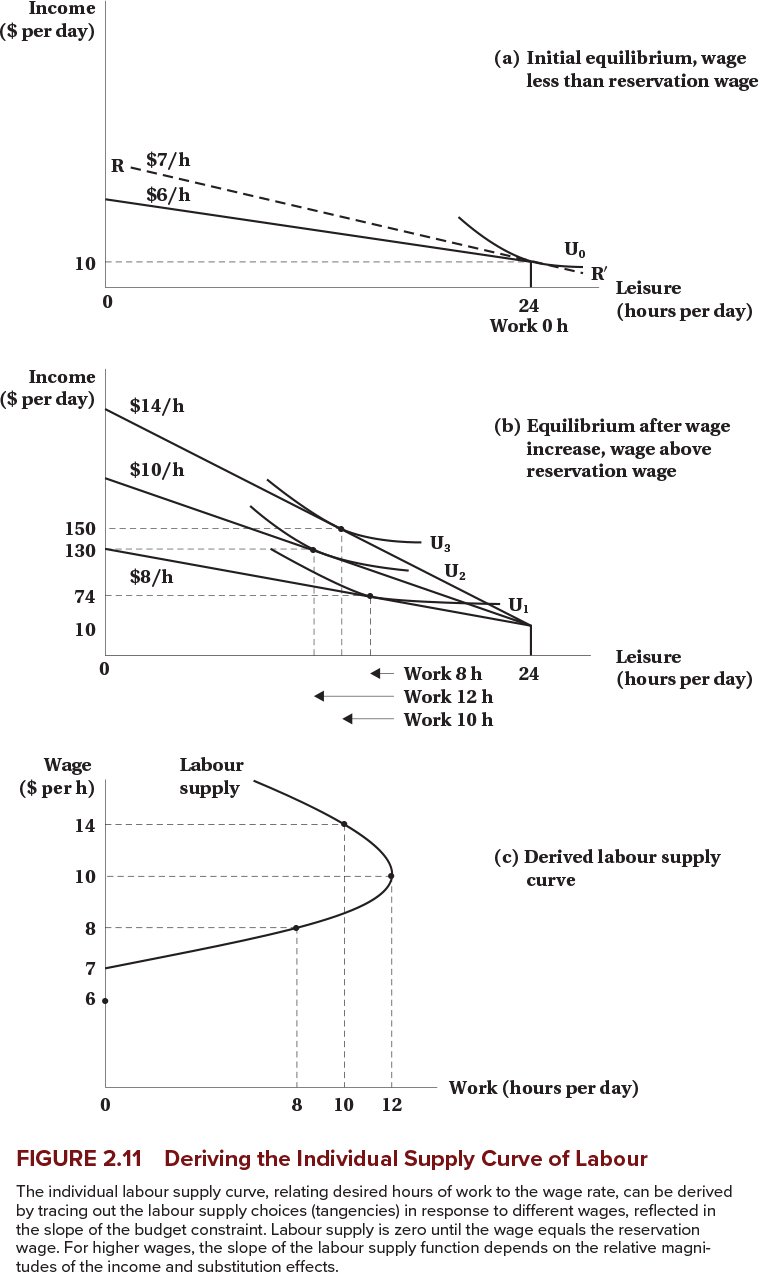
\includegraphics[width=0.3\linewidth]{ben54842_0211}.
\end{frame}

% ============================================================
\section{Evidence and Applications}
% ============================================================

\begin{frame}{Empirical Evidence: What Do We Test?}
\transfade
\begin{enumerate}[<+->]
  \item Does behaviour match the model’s predictions?
  \item How responsive is labour supply to wages?
\end{enumerate}
\tiny {\it Source:} Evidence questions. :contentReference[oaicite:28]{index=28}
\end{frame}

\begin{frame}{TABLE 2.2: Labour Force Participation of Married Women, Canada (2017)}
\transfade
\tiny
\begin{tabular}{lccc}
\toprule
\textbf{Group} & \textbf{Participation Rate} & \textbf{Raw Diff.\ from Base} & \textbf{Adjusted Diff.\ from Base} \\
\midrule
All Women, Total & 75.3 &  &  \\
\midrule
\multicolumn{4}{l}{\textbf{Age}} \\
20--24 (1.1\%) & 89.4 & N/A & N/A \\
25--34 (18.9\%) & 84.4 & --5.0 & --3.7 \\
35--44 (23.9\%) & 85.5 & --3.9 & --3.0 \\
45--54 (24.0\%) & 84.8 & --4.6 & --7.3 \\
55--64 (23.8\%) & 64.8 & --24.6 & --22.3 \\
65--69 (8.4\%) & 27.5 & --61.9 & --52.6 \\
\midrule
\multicolumn{4}{l}{\textbf{Age of youngest child at home}} \\
No children under 18 (60.1\%) & 70.9 & N/A & N/A \\
0--5 years (18.4\%) & 77.4 & 6.5 & --13.9 \\
6--9 years (7.7\%) & 84.6 & 13.7 & --5.4 \\
10--15 years (10.1\%) & 87.0 & 16.1 & --0.7 \\
16--17 years (3.7\%) & 86.3 & 15.4 & 0.2 \\
\midrule
\multicolumn{4}{l}{\textbf{Education}} \\
Less than high school (8.2\%) & 49.6 & N/A & N/A \\
High school/some post-sec (23.6\%) & 67.9 & 18.3 & 12.1 \\
Non-univ post-sec cert (30.7\%) & 77.8 & 28.2 & 18.8 \\
University degree (37.6\%) & 83.7 & 34.1 & 22.4 \\
\midrule
\multicolumn{4}{l}{\textbf{Spouse's income}} \\
None (or negative) (18.0\%) & 49.7 & N/A & N/A \\
\$1--\$9{,}999 (8.7\%) & 62.0 & 12.3 & 7.7 \\
\$10{,}000--\$24{,}999 (9.1\%) & 78.6 & 28.9 & 17.5 \\
\$25{,}000--\$49{,}999 (18.2\%) & 82.3 & 32.6 & 18.4 \\
\$50{,}000--\$74{,}999 (17.1\%) & 87.1 & 37.4 & 21.0 \\
\$75{,}000--\$99{,}999 (12.4\%) & 86.3 & 36.6 & 18.9 \\
\$100{,}000--\$149{,}999 (10.7\%) & 84.2 & 34.5 & 17.1 \\
Over \$150{,}000 (5.7\%) & 74.1 & 24.4 & 7.4 \\
\bottomrule
\end{tabular}

\vspace{0.25em}
\tiny {\it Source:} Table headings/values as shown. :contentReference[oaicite:29]{index=29}
\end{frame}

\begin{frame}{Empirical Elasticities}
\transfade
\textbf{Uncompensated} (Marshallian), \textbf{Compensated} (Hicksian), and \textbf{Income} elasticities summarize responsiveness.\\[0.3em]
Policy uses: predicting hours/participation responses to taxes, transfers, wage changes.

\end{frame}

\begin{frame}{TABLE 2.3: Estimated Elasticities of Labour Supply}
\transfade
\small
\begin{tabular}{lccc}
\toprule
\textbf{Group} & \textbf{Uncompensated Wage} & \textbf{Compensated Wage} & \textbf{Income} \\
\midrule
Both sexes & 0.0 to 0.2 & 0.1 to 0.3 & --0.1 to 0.0 \\
Men and single women & --0.1 to 0.2 & 0.1 to 0.3 & --0.1 to 0.0 \\
Married women & 0.1 to 0.3 & 0.2 to 0.4 & --0.1 to 0.0 \\
\bottomrule
\end{tabular}

\vspace{0.25em}

\end{frame}

% ============================================================
\section{Extensions \& Applications}
% ============================================================

\begin{frame}{Discouraged vs.\ Added Worker Effects}
\transfade
\begin{itemize}[<+->]
  \item \textbf{Discouraged}: High unemployment \(\Rightarrow\) some stop searching \(\Rightarrow\) exit LF (hidden unemployment).
  \item \textbf{Added}: Household income loss \(\Rightarrow\) others enter LF to offset.
\end{itemize}

\end{frame}

\begin{frame}{Moonlighting, Overtime, Flexible Hours}
\transfade
\begin{itemize}[<+->]
  \item Why work a second job at a lower wage? (Hours constraints / underemployment.)
  \item Why an overtime \textit{premium}? (To induce hours beyond the preferred level.)
  \item Flex-time/compressed weeks can improve matches and reduce costs.
\end{itemize}

\end{frame}

\begin{frame}{Figure 2.12: Fixed Hours Constraint, Underemployment, Moonlighting }
\centering
\vspace{1.7em}

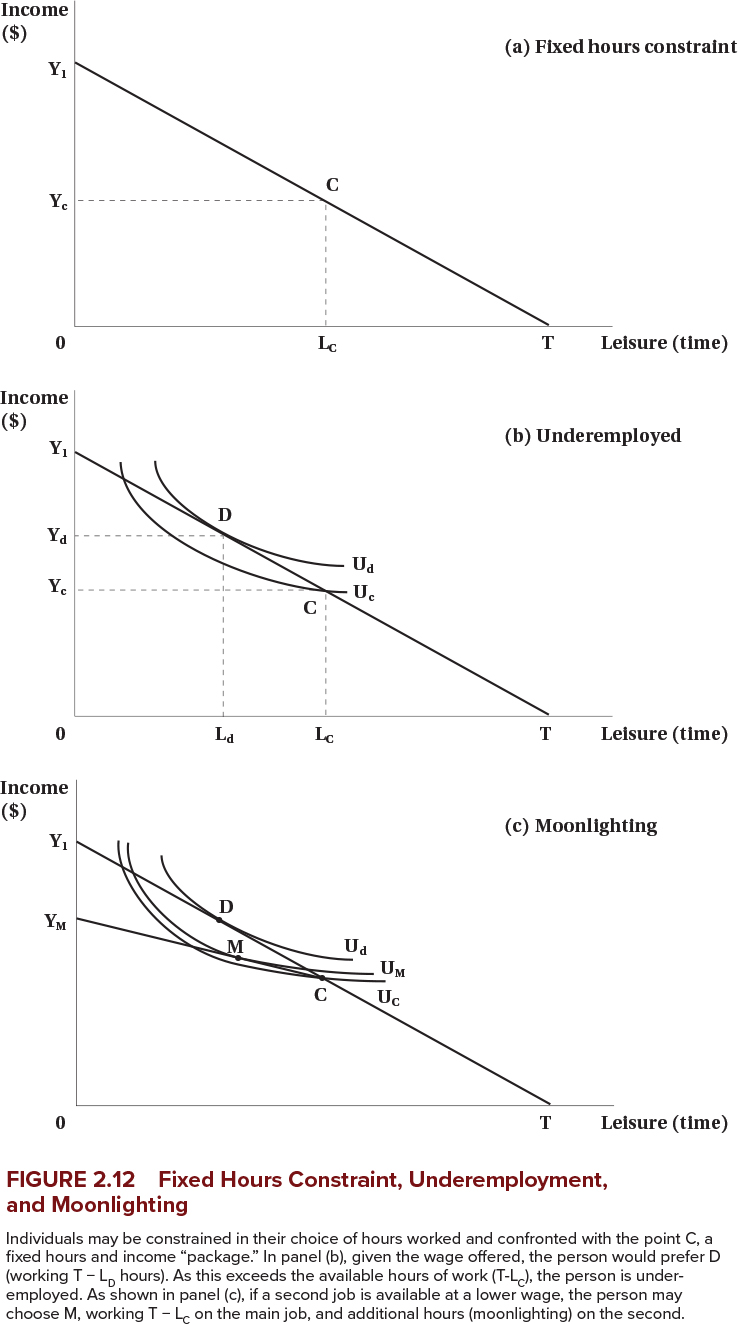
\includegraphics[width=0.29\linewidth]{ben54842_0212}.

\end{frame}

\begin{frame}{Overtime and Overemployment}
\transfade
\begin{itemize}[<+->]
  \item Workers may prefer fewer hours at the going wage.
  \item Overtime \textbf{premium} compensates disutility of extra hours and aligns supply with firm demand.
\end{itemize}

\end{frame}

\begin{frame}{Figure 2.13: Overemployment and Overtime}
\centering
\vspace{2.6em}

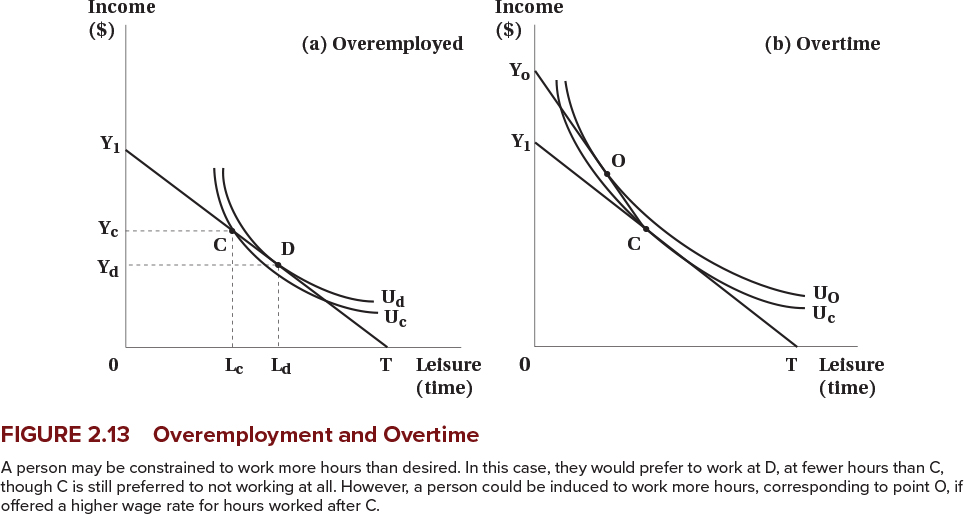
\includegraphics[width=0.98\linewidth]{ben54842_0213}.
\end{frame}

\begin{frame}{Figure 2.14: Overtime Premium vs.\ Straight-Time Equivalent}
\centering
\vspace{2em}

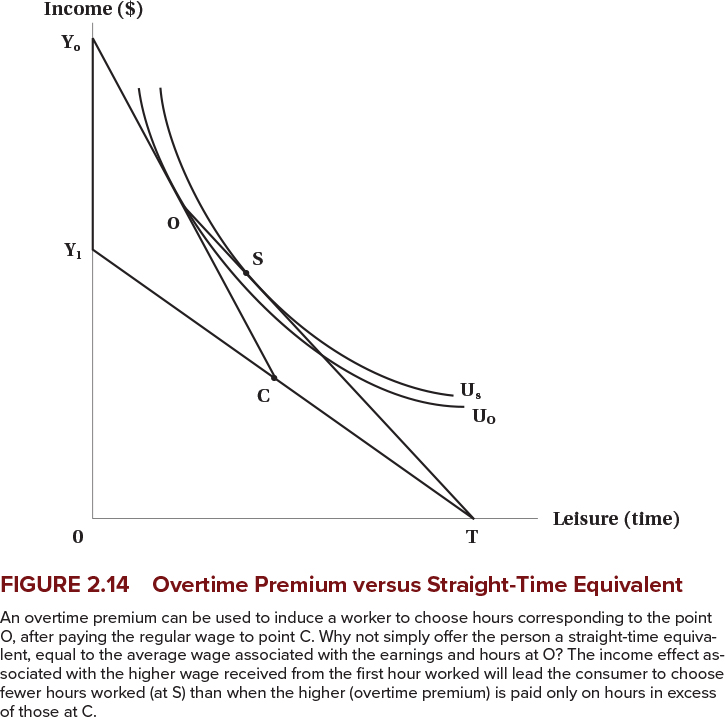
\includegraphics[width=0.58\linewidth]{ben54842_0214}.

\end{frame}

\begin{frame}{Choice in Working Hours}
\transfade
\begin{itemize}[<+->]
  \item Heterogeneous preferences over schedules across groups.
  \item Allowing desired hours can reduce turnover and training costs.
\end{itemize}

\end{frame}

\begin{frame}{Figure 2.15: Gains from Alternative Work Schedules }
\centering
\vspace{2em}

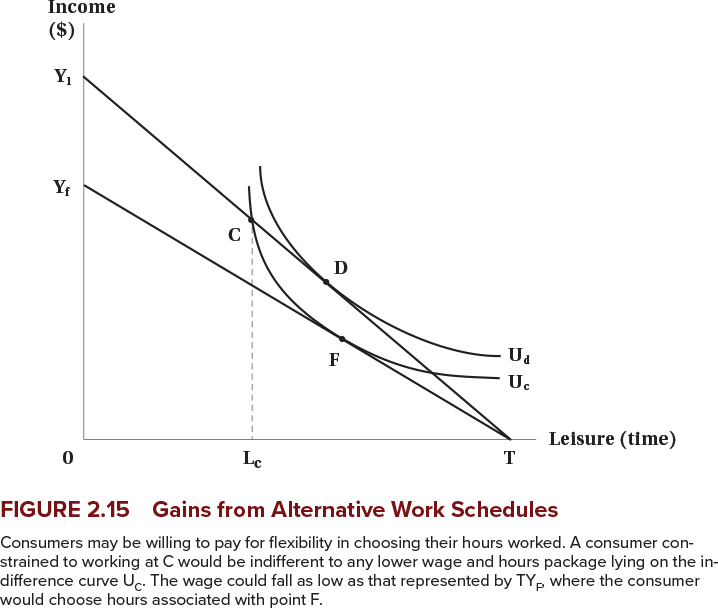
\includegraphics[width=0.65\linewidth]{ben54842_0215}.

\end{frame}

% ============================================================
\section{Chapter Summary}
% ============================================================

\begin{frame}{Summary (1/2)}
\transfade
\begin{itemize}[<+->]
  \item Attachment has two margins: \textbf{participation} and \textbf{hours}.
  \item The consumer choice model captures both: choose income (consumption) and leisure within a potential income constraint.
  \item \textbf{Reservation wage} governs participation: above it \(\Rightarrow\) work; below it \(\Rightarrow\) no participation.
\end{itemize}

\end{frame}

\begin{frame}{Summary (2/2)}
\transfade
\begin{itemize}[<+->]
  \item Varying the wage traces an individual’s labour supply; income vs.\ substitution effects can bend supply backward.
  \item Applications include added worker effects, overtime premiums, and the value of flexible schedules.
\end{itemize}

\end{frame}

% ============================================================
\begin{frame}
\centering
\Huge{\textbf{Thank You!}} \\

\end{frame}

\end{document}
